% -*- LaTeX -*-
% -*- coding: utf-8 -*-
%
% michael a.g. aïvázis
% california institute of technology
% (c) 1998-2012 all rights reserved
%

\section{Two simple implementations}
\label{sec:simple}

Turning the math of the previous section into actual code is not very hard, especially if
you don't try improve the effective convergence rate by sampling the integration region in
tricky ways. To simplify things even further, we will forgo integration with non-trivial
integrands for now. Instead, we will compute areas and volumes by letting $f$ be the unit
function over our chosen region.
%
\begin{figure}
\centering
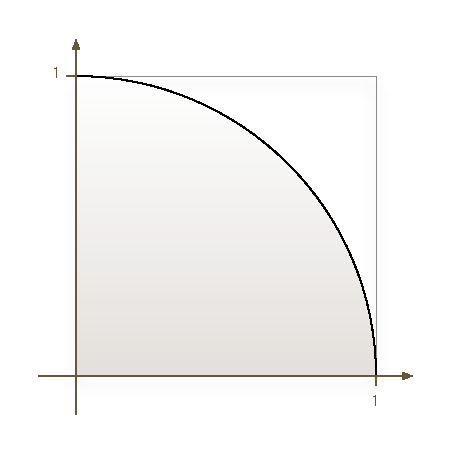
\includegraphics[scale=.75]{figures/quadrant.pdf}
\caption{Estimating $\pi$ by computing the area of a quadrant of the unit circle
  \label{fig:pie}}
\end{figure}
%

As a warm up exercise, let's use Monte Carlo integration to compute $\pi$. We can get an
estimate for $\pi/4$ by computing the area of the upper right quadrant of the unit circle,
as shown in \figref{pie}. This will require generating points in the unit square and
counting the fraction that fall in the shaded region.

The implementation strategy is very simple. Let $N$ be the total number of points we would like
to generate. We will set up two counters, $t$ for the total number of points and $i$ for the
points that fall inside the unit circle, and iterate $N$ times building random points in the
unit square, checking whether each point falls inside the unit circle and updating our counters
appropriately, as shown in \algref{pi}.  Integration has been reduced to placing points in two
bins. Note that $\Theta(\Omega)$ in \eqref{mc} corresponds to the conditional in
\alglineref{pi:check}, and the dimensionality of the integrand is reflected in the number of
calls to the random number generator it takes to build a point. Further, our sampling box $B$
has unit area, so there is no need for any extra normalization of the result.
% 
\begin{algorithm}
\caption{$\pi_{N}$: the Monte Carlo estimate of $\pi$ \label{alg:pi}}
%
\DontPrintSemicolon
\SetAlgoNoEnd
%
$i \leftarrow 0$ \;
$t \leftarrow 0$ \;
\While{$t < N$}{
   $x \leftarrow \mbox{random()}$ \;
   $y \leftarrow \mbox{random()}$ \;
   \If{$\sqrt{x^{2}+y^{2}} \leq 1$}{ \nllabel{line:pi:check}
      $i \leftarrow i + 1$
   }
   $t \leftarrow t + 1$
}
$\pi_{N} = 4 i/N \;$ %\frac{i}{t}$ \;
\end{algorithm}
%

It is straightforward to generalize this procedure to compute integrals of non-trivial
integrands over higher dimensional regions. Perhaps you can already see that computing the
integral of a non-trivial $f$ should only affect our interpretation of the counter $i$. We will
address this and other ways to generalize this algorithm in \secref{classes}.

\subsection{The two-minute python script}
\label{sec:simple:python}

The python implementation is a straightforward translation of the pseudocode of
\algref{pi}. The python standard library\supercite{python-doc} includes the package {\tt random}
with an implementation of the Mersenne Twister\supercite{mersenne-twister} random number
generator. Two minutes of typing produce:
%
\python{
  % firstnumber=9,
  linerange={9-25},
  label={lst:simple:python},
  caption={\srcfile{simple/gauss.py}: Estimating $\pi$ in python},
}{listings/simple/gauss.py}
%
Note that by deciding whether the point is inside the circle using the square of the distance
saves us a large number of calls to \function{sqrt}. This type of consideration is ubiquitous
when trying to get good performance out of Monte Carlo methods.  Also, note that we did not
have to convert our integer counters to floats before the computation of the area fraction,
since division of integers results in floating point numbers whenever necessary, a behavior
that is standard since version 3.0 of the python interpreter.

There are two obvious questions to answer: how accurate and how fast is this calculation?  To
answer these questions, we can perform some experiments where we vary the total number of
points $N$, and record the result and the time it took, as shown in \tabref{simple-python}.
%
\begin{table}
\centering
\[
\begin{array}{rd{8}cd{4}}
% headersep
  \multicolumn{1}{c}{N} & 
  \multicolumn{1}{c}{\pi_{N}} & 
  \multicolumn{1}{c}{\Delta} & 
  \multicolumn{1}{c}{t \mbox{(sec)}} \\
  \hline \\ [-1.5ex]
% body
  10^{0} &  0          & 1                   &    .014  \\
  10^{1} &  3.6        & 1.46 \times 10^{-1} &    .014  \\
  10^{2} &  3.36       & 6.95 \times 10^{-2} &    .014  \\
  10^{3} &  3.076      & 2.09 \times 10^{-2} &    .015  \\
  10^{4} &  3.156      & 4.59 \times 10^{-3} &    .027  \\
  10^{5} &  3.14496    & 1.07 \times 10^{-3} &    .144  \\
  10^{6} &  3.144028   & 7.75 \times 10^{-4} &   1.265  \\
  10^{7} &  3.142112   & 1.65 \times 10^{-4} &  12.624  \\
  10^{8} &  3.14170136 & 3.46 \times 10^{-5} & 130.430 
\end{array}
\]
\caption{Estimating $\pi$: accuracy and cost of the python implementation
  \label{tab:simple-python}}
\end{table}
%
Varying the sample size involves editing the script, making the corresponding change to the
value of $N$ and making another run. We could have exposed this variable to the end user by
attaching it to a command line argument, but there is no reason to go through all this at this
point. We will see a better way to get this kind of flexibility in \secref{pyreapp}.

As estimators of $\pi$ go, this is not a good one: it converges rather slowly and it is rather
expensive. Sample sets larger than $10^{8}$ are not practical in pure python. How much better
can we do by switching over to a lower level language, such as \cpp?

\subsection{The ten-minute \cpp\ program}
\label{sec:simple:c}

The implementation in \cpp\ is also fairly straightforward. One complication is that the random
number generator in the standard \cc\ library has rather poor properties and it is not well
suited for stochastic calculations; fortunately, \package{GSL}, the \package{GNU} Scientific
Library\supercite{gsl}, has a large number of good generators whose properties and cost are
rather well documented. Binary distributions of \package{GSL} are available for a variety of
platforms, and you can always download and compile it from its freely available source code.

Note that we are only using \cpp\ as a better \cc, taking advantage of the strict type
checking, the ability to declare variables where we need them, and the prettier comment
syntax. Later we will see a couple of other reasons to compile \cc\ programs with \cpp\
compilers. For now, here is what a simple translation of the pseudocode of \algref{pi} looks
like:
%
\Cpp{
  % firstnumber=9,
  linerange={9-35},
  label={lst:simple:cpp},
  caption={\srcfile{simple/gauss.cc}: Estimating $\pi$ in \cpp},
}{listings/simple/gauss.cc}
%
whose accuracy and cost is shown in \tabref{simple-c}. It is clear that the
\cpp\ implementation is almost an order of magnitude faster. However, the cost of making the
necessary changes to the value of $N$ is a little higher for the \cpp\ program, since the cycle
involves the additional steps of compiling and linking. Again, a flexible program would expose
this variable to the end user; we will address this issue in \secref{pyreapp}.
%
\begin{table}
\centering
\[
\begin{array}{rd{8}cd{4}}
% headers
  \multicolumn{1}{c}{N} & 
  \multicolumn{1}{c}{\pi_{N}} & 
  \multicolumn{1}{c}{\Delta} & 
  \multicolumn{1}{c}{t \mbox{(sec)}} \\
  \hline \\ [-1.5ex]
% body
  10^{0} &  0          & 1                   &    .002  \\
  10^{1} &  3.2        & 1.86 \times 10^{-2} &    .002  \\
  10^{2} &  3.16       & 5.86 \times 10^{-3} &    .002  \\
  10^{3} &  3.2        & 1.86 \times 10^{-2} &    .002  \\
  10^{4} &  3.1456     & 1.28 \times 10^{-3} &    .004  \\
  10^{5} &  3.13528    & 2.01 \times 10^{-3} &    .026  \\
  10^{6} &  3.140756   & 2.66 \times 10^{-4} &    .230  \\
  10^{7} &  3.141948   & 1.13 \times 10^{-4} &   2.277  \\
  10^{8} &  3.1417769  & 5.86 \times 10^{-5} &  22.749  \\
  10^{9} &  3.1415631  & 9.41 \times 10^{-6} & 227.735   
\end{array}
\]
\caption{Estimating $\pi$: accuracy and cost of the \cpp\ implementation
  \label{tab:simple-c}}
\end{table}
%

We have chosen the \package{RANLUX} random number generator, one the most costly but well behaved
generators in the library. Even so, the \cpp\ implementation is six to seven times
faster. Since the python generator \function{random} is implemented in \cc, the difference in
running times is mostly due to the cost of setting up the function call in the two
languages. For many computations, the extra flexibility that python has to offer is worth the
performance hit; for others it is unacceptable. However, as we will see later, a little care,
some common sense, and some careful profiling will make it possible to have the best of both
worlds.

% end of file 
